%%%%%%%%%%%%%%%%%%%%%%%%%%%%%%%%%%%%%%%%%%%%%%%%%%%%%%%%%%
\frame {\frametitle{Spark Schedulers}
%%%%%%%%%%%%%%%%%%%%%%%%%%%%%%%%%%%%%%%%%%%%%%%%%%%%%%%%%%
\begin{itemize}
	\item {\bf Two main scheduler components, executed by the driver}
	\begin{itemize}
		\item The DAG scheduler
		\item The Task scheduler
	\end{itemize}

	\vspace{20pt}

	\item {\bf Objectives}
	\begin{itemize}
		\item Gain a broad understanding of how Spark submits Applications
		\item Understand how \textit{Stages} and \textit{Tasks} are built, and their optimization
		\item Understand interaction among various other Spark components
	\end{itemize}
\end{itemize}
}

%%%%%%%%%%%%%%%%%%%%%%%%%%%%%%%%%%%%%%%%%%%%%%%%%%%%%%%%%%
\frame {\frametitle{Submitting a Spark Application: A Walk Through}
%%%%%%%%%%%%%%%%%%%%%%%%%%%%%%%%%%%%%%%%%%%%%%%%%%%%%%%%%%
\begin{figure}[h]
  \centering
  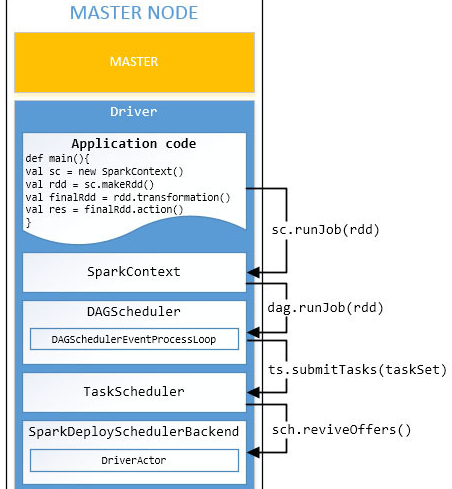
\includegraphics[scale=0.45]{./Figures/submit_modules}
  \label{fig:spark_submit_modules}
\end{figure}
}

%%%%%%%%%%%%%%%%%%%%%%%%%%%%%%%%%%%%%%%%%%%%%%%%%%%%%%%%%%
\frame {\frametitle{Submitting a Spark Application: Details}
%%%%%%%%%%%%%%%%%%%%%%%%%%%%%%%%%%%%%%%%%%%%%%%%%%%%%%%%%%
\begin{columns}[t, onlytextwidth]
	\column[T]{.5\textwidth}
		
			\begin{figure}[h]
			  \centering
			  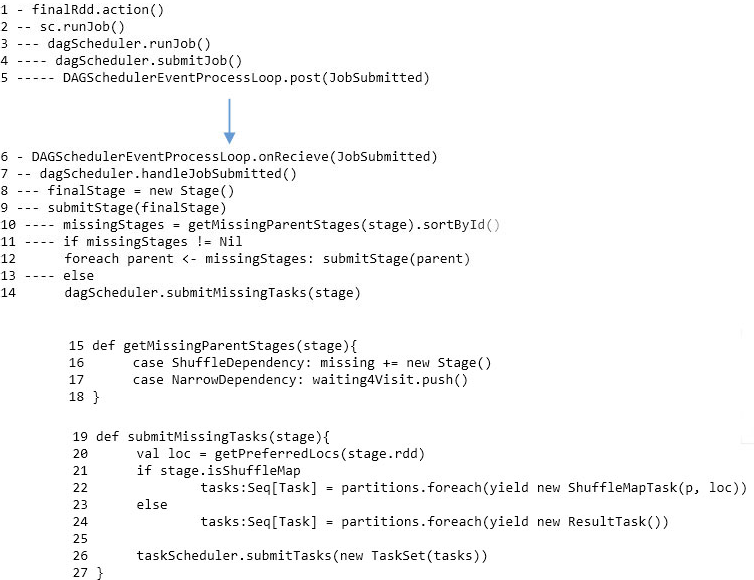
\includegraphics[scale=0.3]{./Figures/submit_stack_1}
			  \label{fig:spark_caching_workers}
			\end{figure}
	
	\column[T]{.5\textwidth}
		
			\begin{figure}[h]
			  \centering
			  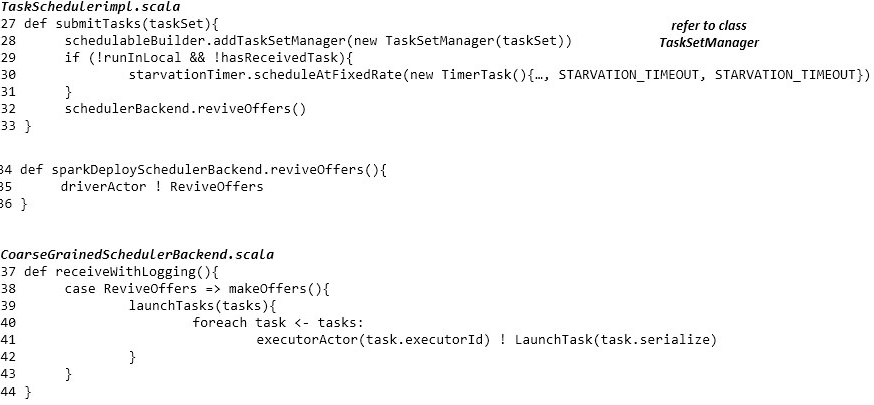
\includegraphics[scale=0.3]{./Figures/submit_stack_2}
			  \label{fig:caching_stack_calls}
			\end{figure}

\end{columns}
}

%%%%%%%%%%%%%%%%%%%%%%%%%%%%%%%%%%%%%%%%%%%%%%%%%%%%%%%%%%
\frame {\frametitle{The DAG Scheduler}
%%%%%%%%%%%%%%%%%%%%%%%%%%%%%%%%%%%%%%%%%%%%%%%%%%%%%%%%%%
\begin{itemize}
	\item {\bf Stage-oriented scheduling}
	\begin{itemize}
		\item Computes a DAG of stages for each job in the application
		\item[] \texttt{Lines 10-14}, details in \texttt{Lines 15-27}
		\item Keeps track of which RDD and stage output are materialized
		\item Determines an optimal schedule, minimizing stages
		\item Submit stages as sets of Tasks (\texttt{TaskSets}) to the Task scheduler
		\item[] \texttt{Line 26}
	\end{itemize}

	\item {\bf Data locality principle}
	\begin{itemize}
		\item Uses ``preferred location'' information (optionally) attached to each RDD
		\item[] \texttt{Line 20}
		\item Package this information into Tasks and send it to the Task scheduler
	\end{itemize}

	\item {\bf Manages Stage failures}
	\begin{itemize}
		\item Failure type: (intermediate) data loss of shuffle output files
		\item Failed stages will be resubmitted
		\item NOTE: Task failures are handled by the Task scheduler, which simply resubmit them if they can be computed with no dependency on previous output
	\end{itemize}

\end{itemize}
}

%%%%%%%%%%%%%%%%%%%%%%%%%%%%%%%%%%%%%%%%%%%%%%%%%%%%%%%%%%
\frame {\frametitle{The DAG Scheduler: Implementation Details}
%%%%%%%%%%%%%%%%%%%%%%%%%%%%%%%%%%%%%%%%%%%%%%%%%%%%%%%%%%
\begin{itemize}
	\item {\bf Implemented as an event queue}
	\begin{itemize}
		\item Uses a daemon thread to handle various kinds of events
		\item[] \texttt{Line 6}
		\item \texttt{JobSubmitted}, \texttt{JobCancelled}, \texttt{CompletionEvent}
		\item The thread ``swipes'' the queue, and routes event to the corresponding handlers
	\end{itemize}

	\vspace{10pt}

	\item {\bf What happens when a job is submitted to the DAGScheduler?}
	\begin{itemize}
		\item \texttt{JobWaiter} object is created
		\item \texttt{JobSubmitted} event is fired
		\item The daemon thread blocks and wait for a job result
		\item[] \texttt{Lines 3,4}
	\end{itemize}

\end{itemize}
}

%%%%%%%%%%%%%%%%%%%%%%%%%%%%%%%%%%%%%%%%%%%%%%%%%%%%%%%%%%
\frame {\frametitle{The DAG Scheduler: Implementation Details (2)}
%%%%%%%%%%%%%%%%%%%%%%%%%%%%%%%%%%%%%%%%%%%%%%%%%%%%%%%%%%
\begin{itemize}
	\item {\bf Who handles the \texttt{JobSubmitted} event?}
	\begin{itemize}
		\item Specific handler called \texttt{handleJobSubmitted}
		\item[] \texttt{Line 6}
	\end{itemize}


	\item {\bf Walk-through to the Job Submitted handler}
	\begin{itemize}
		\item Create a new job, called \texttt{ActiveJob}
		\item New job starts with only 1 stage, corresponding to the last stage of the job upon which an action is called
		\item[] \texttt{Lines 8-9}
		\item Use the dependency information to produce additional stages
		\begin{itemize}
			\item Shuffle Dependency: create a new map stage
			\item[] \texttt{Line 16}
			\item Narrow Dependency: pipes them into a single stage
			\item[] \texttt{getMissingParentStages}
		\end{itemize}
	\end{itemize}
\end{itemize}
}

%%%%%%%%%%%%%%%%%%%%%%%%%%%%%%%%%%%%%%%%%%%%%%%%%%%%%%%%%%
\frame {\frametitle{More About Stages}
%%%%%%%%%%%%%%%%%%%%%%%%%%%%%%%%%%%%%%%%%%%%%%%%%%%%%%%%%%
\begin{itemize}
	\item {\bf What is a DAG}
	\begin{itemize}
		\item Directed acyclic graph of stages
		\item Stage boundaries determined by the shuffle phase
		\item Stages are run in \emph{topological order}
	\end{itemize}

	\item {\bf Definition of a Stage}
	\begin{itemize}
		\item Set of \emph{independent} tasks
		\item All tasks of a stage apply the same function
		\item All tasks of a stage have the same dependency type
		\item All tasks in a stage belong to a \texttt{TaskSet}
	\end{itemize}

	\item {\bf Stage types}
	\begin{itemize}
		\item Shuffle Map Stage: stage tasks results are inputs for another stage
		\item Result Stage: tasks compute the final action that initiated a job (e.g., \texttt{count()}, \texttt{save()}, etc.)
	\end{itemize}

\end{itemize}
}

%%%%%%%%%%%%%%%%%%%%%%%%%%%%%%%%%%%%%%%%%%%%%%%%%%%%%%%%%%
\frame {\frametitle{The Task Scheduler}
%%%%%%%%%%%%%%%%%%%%%%%%%%%%%%%%%%%%%%%%%%%%%%%%%%%%%%%%%%
\begin{itemize}
	\item {\bf Task oriented scheduling}
	\begin{itemize}
		\item Schedules tasks for a \emph{single} \texttt{SparkContext}
		\item Submits tasks sets produced by the DAG Scheduler
		\item Retries failed tasks
		\item Takes care of \emph{stragglers} with speculative execution
		\item Produces events for the DAG Scheduler
	\end{itemize}

	\item {\bf Implementation details}
	\begin{itemize}
		\item The Task scheduler creates a \texttt{TaskSetManager} to wrap the \texttt{TaskSet} from the DAG scheduler
		\item[] \texttt{Line 28}
		\item The \texttt{TaskSetManager} class operates as follows:
		\begin{itemize}
			\item Keeps track of each task status
			\item Retries failed tasks
			\item Imposes data locality using \emph{delayed scheduling}
			\item[] \texttt{Lines 29,30}
		\end{itemize}
		\item Message passing implemented using \emph{Actors}, and precisely using the \emph{Akka framework}
	\end{itemize}
\end{itemize}
}

%%%%%%%%%%%%%%%%%%%%%%%%%%%%%%%%%%%%%%%%%%%%%%%%%%%%%%%%%%
\frame {\frametitle{Running Tasks on Executors}
%%%%%%%%%%%%%%%%%%%%%%%%%%%%%%%%%%%%%%%%%%%%%%%%%%%%%%%%%%
\begin{columns}[t, onlytextwidth]
	\column[T]{.3\textwidth}
		
			\begin{figure}[h]
			  \centering
			  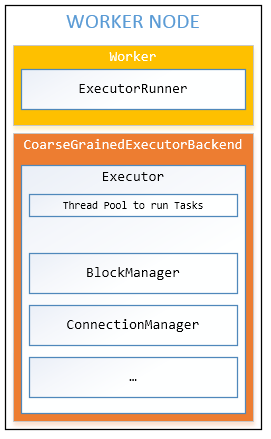
\includegraphics[scale=0.5]{./Figures/executor_components}
			  \label{fig:spark_caching_workers}
			\end{figure}
	
	\column[T]{.7\textwidth}
		
			\begin{figure}[h]
			  \centering
			  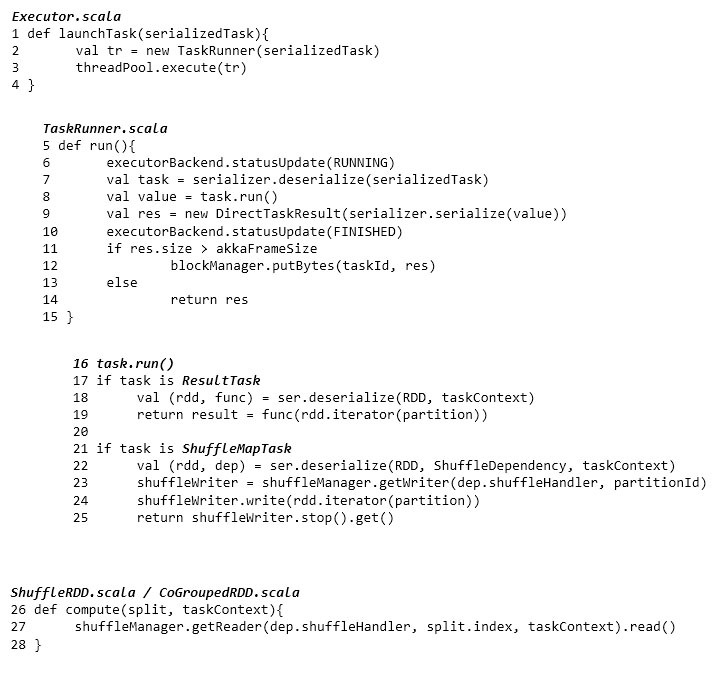
\includegraphics[scale=0.4]{./Figures/executor_stack}
			  \label{fig:caching_stack_calls}
			\end{figure}

\end{columns}
}

%%%%%%%%%%%%%%%%%%%%%%%%%%%%%%%%%%%%%%%%%%%%%%%%%%%%%%%%%%
\frame {\frametitle{Running Tasks on Executors}
%%%%%%%%%%%%%%%%%%%%%%%%%%%%%%%%%%%%%%%%%%%%%%%%%%%%%%%%%%
\begin{itemize}
	\item {\bf Executors run two kinds of tasks}
	\begin{itemize}
		\item \texttt{ResultTask}: apply the action on the RDD, once it has been computed, alongside all its dependencies
		\item[] \texttt{Line 19}
		\item \texttt{ShuffleTask}: use the Block Manager to store shuffle output using the \texttt{ShuffleWriter}
		\item[] \texttt{Lines 23,24}
		\item The \texttt{ShuffleRead} component depends on the type of the RDD, which is determined by the compute function and the transformation applied to it
	\end{itemize}
\end{itemize}
}
